
\documentclass[11pt]{article}
\usepackage{cs65f10}
\usepackage{times}
\usepackage{latexsym}
\usepackage{graphics}
\usepackage{smiley}
\setlength\titlebox{6.5cm}    % Expanding the titlebox
\title{Analyzing the Relationship Between Tweets, Box-Office Performance, and Stocks}

% Alter some LaTeX defaults for better treatment of figures:
    % See p.105 of "TeX Unbound" for suggested values.
    % See pp. 199-200 of Lamport's "LaTeX" book for details.
    %   General parameters, for ALL pages:
    \renewcommand{\topfraction}{0.9}	% max fraction of floats at top
    \renewcommand{\bottomfraction}{0.8}	% max fraction of floats at bottom
    %   Parameters for TEXT pages (not float pages):
    \setcounter{topnumber}{2}
    \setcounter{bottomnumber}{2}
    \setcounter{totalnumber}{4}     % 2 may work better
    \setcounter{dbltopnumber}{2}    % for 2-column pages
    \renewcommand{\dbltopfraction}{0.9}	% fit big float above 2-col. text
    \renewcommand{\textfraction}{0.07}	% allow minimal text w. figs
    %   Parameters for FLOAT pages (not text pages):
    \renewcommand{\floatpagefraction}{0.7}	% require fuller float pages
	% N.B.: floatpagefraction MUST be less than topfraction !!
    \renewcommand{\dblfloatpagefraction}{0.7}	% require fuller float pages

	% remember to use [htp] or [htpb] for placement

\author{Catie Meador\\
  Swarthmore College\\
  500 College Ave\\
  Swarthmore PA 19081\\
  {\tt cmeador1@cs.swarthmore.edu}  
  \And
  Jonathan Gluck\\
  Swarthmore College\\
  500 College Ave\\
  Swarthmore PA 19081\\
  {\tt jgluck1@cs.swarthmore.edu}  
}

\date{}

\begin{document}
\maketitle

\begin{abstract}
Sentiment analysis, a powerful tool determining public opinion, is often applied to corpora of full length documents. Guided by recent forays into sentiment analysis on micro-blogging platforms, we will examine popular opinion of movies and stocks and compare them to real world indicators of popularity(e.g: box office.)
\end{abstract}

\section{Introduction}

The microblogging site Twitter is a social networking service in which users, of which there are currently over 224 million, post status updates of 140 characters or less, about anything from their plans for the day to how they feel about the latest version of the iPhone.\cite{dsouza-2010}  Using these updates, or tweets, we propose a method in which, through sentiment analysis, we can determine the opinions of twitter users on various topics, as well as the general popularity of these topics.  In this paper we focus on the topics of recently released movies and stock market performance.  Twitter is especially appropriate for this research due to the wealth of data present, as it currently receives approximately 95 million tweets per day.\cite{rao-2010}  Also, the brevity of tweets makes this data much simpler to sort through, as tweets are generally simple and to the point, making sentiment analysis much less complicated than it would be on longer, more in-depth movie or product reviews.

By analyzing the popularity of movies and stocks through their mentions on twitter, we can receive real-time data on how many people are discussing what movies or stocks/stock products.  The constancy of the twitter feed can be used to predict how a movie or stock will do based on how many mentions it receives on twitter, and how positive or negative these mentions are.  Essentially, these tweets act as very brief movie or product reviews, providing concise data from which to predict the performance of these movies or products.  Due to the social networking nature of twitter, these \textit{reviews} are also seen by other twitter users, and so presumably the sentiment of each tweet will have an effect on the performance of its subject, as each tweet will influence those who read it in buying or not buying a product.

This data is of interest to both the consumers and the creators of these products in many ways.  A daily or hourly analysis of twitter sentiment on various movies or products could be used by consumers to determine the overall sentiment towards that subject in order to help them decide if it's worth spending money on.  For the companies that create these products, twitter plays an important role in customer satisfaction, as companies can use twitter sentiment to determine how consumers feel about their products.\cite{go-distant}  Negative tweets are especially useful if companies are able to determine the main reason behind this negative sentiment in order to fix it.  Also, if a company is planning to release a new product or movie soon, but that product or movie is not very popular on twitter, the company could infer that they need to advertise more in order to create more buzz about their product.  In terms of stocks, there is the potential for a predictive capability to twitter, as it is reasonable to assume that stocks whose products generate a lot of buzz on twitter will do better than stocks who get little to no mention.

While there are already many forms of customer/movie review services available, twitter is unique in its brevity and constant stream of information, sometimes from mobile sources.  While this may not be the best method for discovering major plot details about a movie or exact specifications of the latest apple gadget, we propose that twitter analysis is one of the simplest ways to gain a basic understanding of the popularity and sentiment of movies, products, and various other things, such as people and events.  By comparing the data we extracted from twitter to actual box-office returns and stock performance, we were able to evaluate the accuracy of this method.  Overall, while twitter does not provide very in-depth analyses of products, it can provide enough information to influence consumers, making this information very useful to companies and consumers alike.

\section{Methods}


\subsection{Data Collection}
We explored several avenues of data collection before deciding upon the winning candidate. At first we attempted to collect data by polling twitter, accessing its search api  and querying for tweets having to do with the subject movies and stocks. This proved problematic, as the search API would only return the latest 1500 tweets.

It was at this point that we were informed helpfully, by Brendan Meeder of From Tweets to Polls: Linking Sentiment to Public Opinion Time Series, that Twitter excels at providing data for the present into the future but, due to the short memory span of the search API, is suboptimal for querying the past. Instead of polling Twitter for the past we made use of the continuous streaming API. This streaming API allows the user to provide a list of tracking terms for which, if any of them are mentioned in a tweet, that tweet will be returned to the user.

We compiled a list of tracking terms for four movies and eight traded companies. The movies were of varied popularity, and the eight companies although well known, hailed from different sectors of the market. The tracking terms, some of which may be seen in Table \ref{tterms1} (for a complete list of search terms, please refer to tables \ref{trackmov} and \ref{trackst} in the Appendix), were chosen to best evoke tweets having to do with market sentiment for their respective topic. The movie tracking terms were often variants on the title, but they could also be names of leading actors or the responsible filming studio. The company tracking terms included the ticker symbol for that company, a flagship product of the company, and sometimes a popular figurehead of the company.

\begin{table*}[htb!]
\centering
\caption{Example Tracking Terms by Overall Topic}
\begin{tabular}{|l|c|}
\hline
 & Tracking Term \\
\hline
Movie & Harry Potter, HP7, Tangled, Pixar, White Material, Isabelle Huppart\\
\hline
Stock & AAPL, iPod, Steve Jobs, NKE, Nike, GOOG, Gmail \\
\hline
\end{tabular}
\label{tterms1}
\end{table*}

These streaming requests were allowed to sit for five weeks, accumulating tweets all the while, until we had acquired a corpus of over 2.5 million movie related tweets and over 7.9 million stock related tweets. This inequality in count, taken at face value, might suggest that twitter has more corporate traffic than it does personal; however, it should not be misconstrued in this way. We tracked terms for eight companies, and only four movies; and for each company we had many search terms, while for each movie we had relatively few. 
The tweets were not filtered for language or location, even though these tags do exist in the twitter API. There would have been penalties and many tweets would have slipped by unnoticed as these tags are often not set.

\begin{quote}
Q chaton vou na pre-estreia HP7 mais na sexta eu to la 
\end{quote}

These foreign language tweets should not pose an impact as our sentiment analysis method will ignore them.
\subsection{Tweet Storage}
These tweets were stored in their JSON object format in the order in which they were received. This provided a rough chronological effect as they were received relatively shortly after they had been tweeted. For larger data sets, such as that of Harry Potter, we found it necessary to split the data up into several smaller files.
\subsection{Sentiment Clues}
For this project we made use of two public lists of sentiment words. The first, and more well known, is "The Subjectivity Lexicon" used by Opinion Finder, and in Recognizing Contextual Polarity in Phrase-Level Sentiment Analysis.\cite{wiebe-2005} This is a list of 8200 subjective words labeled with their polarity (positive or negative), their part of speech, and their subjective strength. In addition to these words, we appended a selection of emoticons. Emoticons were used as strong indicators of sentiment in previous work, especially because emoticons are typically unambiguous, so they are one of the most reliable indicators of sentiment.\cite{go-distant}

%\begin{table}[ht!]
%\centering
%\caption{Emoticons as Subjective Clues}
%\begin{tabular}{|l|c|}
%\hline
% & Emoticon \\
%\hline
%Positive & \smiley{wink}, \smiley{happy}, \smiley{alternative},\smiley{smile}\\
%\hline
%Negative & \smiley{sad}, \smiley{crying}, \smiley{angry} \\
%\hline
%\end{tabular}
%\end{table}
\begin{table}[ht!]
\centering
\caption{Emoticons as Subjective Clues}
\begin{tabular}{|l|c|}
\hline
 & Emoticon \\
\hline
Positive & \tt{;)}, \tt{:)}, \tt{:D},\tt{=)}\\
\hline
Negative & \tt{:(}, \tt{:"(}, \tt{:C},\tt{=(}\\
\hline
\end{tabular}
\end{table}

The second list we referenced is used by Twitrattr, an online service which endeavours to determine tangential popular sentiment via twitter. This was a much shorter list of about 150 subjective clues, tailored to better fit the Twitter corpus. One possible advantage to this list was that the words in "The Subjectivity Lexicon" are often overly proper. Twitter is an environment in which there are extremely relaxed grammatical constraints, so presumably the Twittratr list is more applicable.

\begin{quote}
Watching Harry Potter at the movies ft lil brooo
\end{quote}
Twitrattr attempts to create a specialized clue set for a corpus of tweets. This suggests that it may fare better in the long run, being more suited to the tweets we are rating.

\begin{table}[ht!]
\centering
\caption{Juxtaposition of Clue Sets}
\begin{tabular}{|l|c|}
\hline
 & Emoticon \\
\hline
Subjectivity Lex& good, superb, excellent, want\\
\hline
Twitrattr & FTL, pwnd, unusable, hawt\\
\hline
\end{tabular}
\end{table}

In addition to the lists mentioned above, we also edited "The Subjectivity Lexicon" in order to account for instances of the word not.  Typically when not is used in a text, it negates the following sentiment, such as the phrase "not good", which negates the positive sentiment of good and creates a negative sentiment. To account for this we created a duplicate list from "The Subjectivity Lexicon", and then added "not-" to the beginning of each word and flipped the recorded sentiment polarity for these words.  This way, we were able to search the twitter data for instances of "not-" words in addition to normal sentiment words in order to more accurately determine the sentiment of the tweets.

\section{Subjective Mood Analysis}
We took this corpus of tweets and derived a subjective score for each tweet. This allowed us to determine the overall mood on a topic for a given day in which we had collected data. If there was a day in which there were many positive tweets about Steve Jobs, the CEO of Apple Computer inc, it would indicate that public sentiment towards Apple on that day was more positive than normal, and that as a result the stock might be more popular and do well.

\subsection{Tweet Analysis}
We scored the tweets by examining each one in turn. For each tweet we took the frequency of each subjective clue $c_{n}$ from $1$ to $n$ and multiplied that by its polarity, the polarity of a subjective clue being +1 or -1. We then summed this number and arrived at a total subjective score $s$ for a given tweet. This may be seen below:

\begin{equation}
s\ = \sum_{1}^{n}(freq(c_{n})*polarity(c_{n}))
\end{equation}

In addition, we recorded the positive and negative scores separately for each tweet, in case we will want to analyze one mood at a time.

This method of tweet analysis required some supervision of our subjective clue set. For the Disney Pixar movie, Tangled, the tweets were over-penalized, as "tangled" was a negative polarity subjective clue in the OpinionFinder lexicon. These inappropriate clues were removed from the set entirely.

\subsection{Analysis of Negated Clues}
One oversight of the above method for analyzing tweets is that it fails to account for negation. For instance we may look at the tweet below:

\begin{quote}
Hmm... so far i'm not impressed with Tangled music...
\end{quote}

When analyzed without negation, this tweet is marked as positive due to its inclusion of the word "impressed;" however, this tweet strongly expresses a negative sentiment. We sought to address this oversight by adding negated subjectivity clues into our clue set. For each clue "x" in each clue set, we created a new rule "not-x" which had a flipped subjective polarity. When analyzing the tweets we also kept a second copy of the text which replaced every instance of "not\ " with "not-". This allowed the above algorithm to work, conscious of negation. While this method fails to account for all properties of not (for instance, the phrase "not very good" would still be categorized as a positive sentiment), it does take care of the most common instances, without over correcting.  Overall, this method is good because it is simple, but still effective in the distinction of not phrases.

\subsection{Daily Subjectivity Scores}
We scored the overall sentiment in a given day for a given topic by examining all of the scored tweets in that day. We acquired the daily sentiment score $f_{d}$ in two ways. The first of these two methods, which will be known as \textit{excited sentiment score}, may be seen below, where $n$ is the number of tweets in day $d$ and $positive_{n}$ and $negative_{n}$ stand for the number of positive words and negative words, respectively, in tweet $n$:
\begin{equation}
f_{d}\ =\ \frac{\sum_{1}^{n}(positive_{n})}{\sum_{1}^{n}(|negative_{n}|)}
\end{equation}
This indicates that if there were a particularly negative day for a given topic, the daily sentiment score $f_{d}$, would be below 1. We sum over the absolute value of negativeness because negativeness is stored as a negative number.

The second method of finding the daily sentiment score $f$, \textit{known as the basic sentiment score}, was dependent more on tweet count rather than positiveness. It may be seen below, where $count(positive)$ stands for the count of tweets with at least one positive word, and $count(negative)$ stands for the count of tweets with at least one negative word:
\begin{equation}
f_{d}\ =\ \frac{count(positive)}{count(negative)}
\end{equation}
This second method gave rise to an issue where many positive tweets contain both positive and negative words, negating its effect on the daily sentiment score. It is included, however, in the belief that it will still correctly identify overall positivity and negativity.


\section{Results}
After having gathered data over the period of November 16th to December 11th, we halted our streaming request. We amassed a total of $2,762,704$ tweets related to movies, and $4,276,672$ tweets related to stocks and products. The movie tweets were overwhelmingly related to Harry Potter in some way. This has to do with the fact that the first half of the final movie in the 24 billion dollar intellectual property giant. Its tweets eclipsed those of the other movies, as might have been expected. We found that the tweet corpus for Heartless was highly diluted with unrelated tweets and as a result, we will not put too much analysis into that movie. The corporate tweets were taken from a smaller time period, due to difficulty and this might have biased the data.
%(http://business.timesonline.co.uk/tol/business/movers_and_shakers/article3663197.ece)

\subsection{Movie Analysis}
For all of the below we make use of the Opinion Finder clue set, as the twitrattr clue set did not return significantly different results, often ending with a $+/-.01$ to correlation but as to which, it was inconsistent.
\subsubsection{Box Office}
When analyzing each of the movies we compared our gathered data and results against several factors indicative of that movie's success. The most fundamental and widely accepted measure of success we utilized was the box office for each movie. The box office is a measure of the revenue a movie accumulates during a set period of time. In figure \ref{fig:moviebox} you can see the raw number of tweets, hereafter referred to as \textit{tweet throughput}, related to each movie plotted on a logarithmic column graph against each movie's box office, or simply \textit{box}. 
\begin{figure}[ht!]\label{fig:moviebox}
\centering
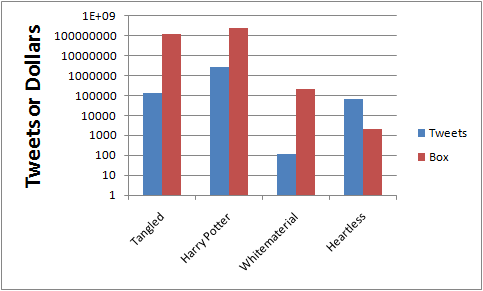
\includegraphics[scale=.60]{img/moviebox.png} 
\caption{Distribution of tweets and box by movie}
\end{figure}
One may see at first glance that there is some relationship between the simple tweet throughput of a movie and its box. Those movies which obtained a higher tweet throughput achieved higher overall boxes. The exception to this rule may be seen in \textit{Heartless}. This is probably due to the higher quantity of noise in the tweet throughput of heartless. A majority of the tweets had little to nothing to do with the movie. This was due to a flaw in the tracking terms used for Heartless; any tweet containing the title of the movie was recorded. This caused every use of the word heartless to be recorded. This should help explain why the higher tweet throughput of heartless doesn't translate to a higher box. Even with this exception, the correlation of tweet throughput to box results is computed with a coefficient of correlation of $r=.91$. 

This exhibits a very strong correlation between the tweet throughput of a given movie and its box. Even if we remove Heartless from the equation that coefficient of correlation only goes up to $r=.92$ Additionally we were interested in examining similarity between tweets and Google queries. After computing the coefficient of correlation between the Google query volume for each movie and the tweet throughput we found the average correlation to be $r=.56$ which jumps to $r=.68$ when heartless is discounted from the equation. This indicates that people in aggregate tend to tweet similar things as those for which they query Google. This may be seen especially in Figure \ref{fig:harrygoog} in which the Google search score fits almost perfectly with the tweet throughput.

These are fascinating correlations for which data can be obtained trivially; however, we want to see how sentiment figures into the picture. In the analysis for \textit{Tangled} we may see some interesting connections which make use of sentiment analysis. In Figure \ref{fig:tangledsimpsent} one may observe both of the sentiment scores we collected. The line above is the daily \textit{excited sentiment score} and the line below is the daily \textit{basic sentiment score}.

\begin{figure}[ht!]
\centering
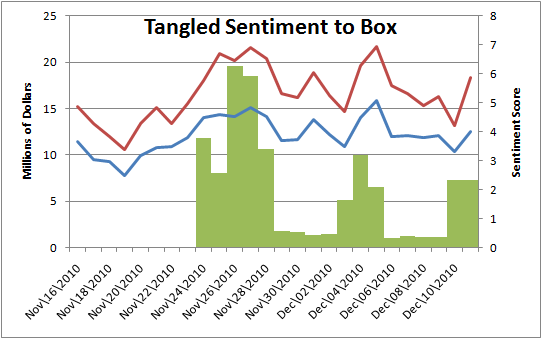
\includegraphics[scale=.6]{img/tangledsimpsent.png} 
\caption{Tangled box to sentiment scores excited above, basic below}
\label{fig:tangledsimpsent}
\end{figure}

At first glance one might notice that there is a relationship between the sentiment scores and the box office. In fact it appears that the sentiment score is shifted slightly rightward so that the sentiment for Tangled the day after is higher when the box office had jumped the day before. This was what we noticed from Figure \ref{fig:tangledsimpsent} and upon calculating the correlation we found that there was a correlation of $r=.66$ between the box office the day before and the basic sentiment score the day after. This was quickly superceded; however, by the correlation $r=.75$ between the box office the day before and the excited sentiment score the day after. This indicated two things, the first is that for Tangled people tended to generate positive tweets about the movie the day after they had seen it, the second is that the excited sentiment score might be a better measure of sentiment than the basic sentiment score.

We then began to examine the results of our negated sentiment clue analysis. These were the tests we had run that were able to identify that the word pair "not bad" implied positive sentiment. The results may be seen below in Figure \ref{fig:tangledsent}. 

\begin{figure}[ht!]
\centering
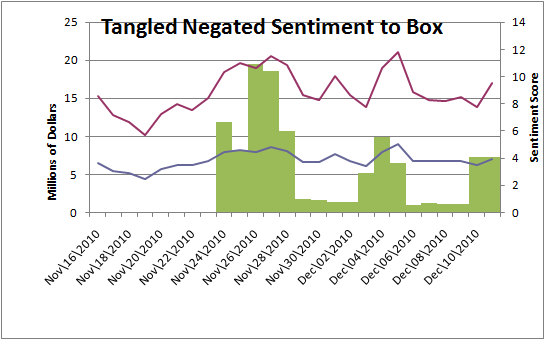
\includegraphics[scale=.55]{img/tangledsent.png} 
\caption{Tangled box to negated sentiment scores excited above, basic below}
\label{fig:tangledsent}
\end{figure}

Similar trends appeared in Figure \ref{fig:tangledsent} as in Figure -\ref{fig:tangledsimpsent}. The pattern that suggested the sentiment score the day after would correlate with the box office the day before was still visible; however, in some places spurious peaks had been smoothed.

 When we calculated the correlations they had increased on all counts. The basic sentiment score the day after the box returned was $r=.68$ while the excited sentiment score the day after the box returned was $r=.78$. Other minor correlations also increased. This was evidence in favor of our negated sentiment analyzer.
 
 While it would be nice to believe that the sentiment scores for a given day would tend to correlate with the box office the night before, this would be a hasty claim. In the instance of Harry Potter, this was not the case. In Figure \ref{fig:hpsent} one may see how  the sentiment related to the box quite differently. 
 
\begin{figure}[ht!]
\centering
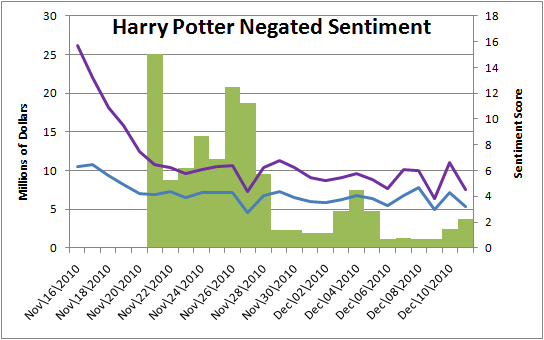
\includegraphics[scale=.55]{img/hpsent.png} 
\caption{Harry Potter box to negated sentiment scores excited above, basic below}
\label{fig:hpsent}
\end{figure}

In the case of Harry Potter it appeared that the sentiment score preceded the box office by a day or so. The resulting correlations were $r=.25$ (basic sentiment day before box), $r=.42$ (excited sentiment day before box), $r=.52$ (basic sentiment two days before box), and $r=.59$ (excited sentiment two days before box). These results suggested that viewers of Harry Potter tweeted their excitement somewhat in advance of their having seen the movie, an interesting disparity to the twitter habits of those who watched Tangled.

This left us with some informative and confusing leads with relation to a movie's tweet throughput and its box. In general, the excited sentiment scores, rather than the basic sentiment scores, seemed be more effective at coaxing a higher correlation across all counts. Additionally, the negated sentiment analysis seemed more effective all around than did the simple analysis. We found that the box correlates consistently with the tweet throughput, but inconsistently with the sentiment scores. This could be because people react differently to different movies. 

Harry Potter was a movie which generated a lot of hype and everyone had high expectations so the tweets reflect that. In the same vein, perhaps Tangled was a movie that struck many as appearing very similar to movies that have been recently released, and thus there was not much hype. In this case the audience might have been pleasantly surprised by the movie and the tweets would relate this after the viewing. Perhaps sentiment score correlations with box office could generate an analysis of movie hype.

\subsubsection{Number of Reviews}
The second variable against which we ran our data was the number of reviews aggregated at Rotten Tomatoes. This being a relative measure of popularity, it correlated very well with the tweet throughput of each movie, with a coefficient of correlation of $r=.93$. The number of reviews also exhibited a strong correlation with the average sentiment score for each movie, producing a correlation of $r=.63$.
\begin{table}[ht!]
\centering
\caption{Movies Reviews and Tweets}
\begin{tabular}{|l|c|c|}
\hline
 Movie & Tweets & Reviews \\
\hline
Tangled& 136062& 115 \\
\hline
Harry Potter & 2559283 & 234\\
\hline
White Material & 121 & 58\\
\hline
Heartless &67238& 33\\
\hline
\end{tabular}
\end{table}

\subsubsection{Tomato Score}
The third variable against which we ran our data was the tomato score, from Rotten Romatoes. The tomato score is an aggregate rating of a movie's "freshness" (read: view worthiness).It is compiled from reviews of professional movie critics from across the media. This score should be roughly analogous to sentiment, as the average sentiment for a movie should hopefully add up to resemble its tomato score, its \textit{view worthiness}. We may see this relationship in Figure \ref{fig:tscoretos}.
\begin{figure}[ht!]
\centering
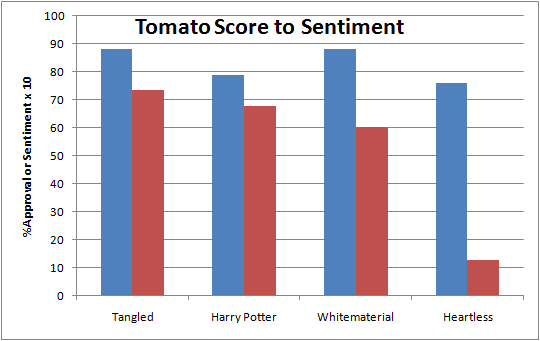
\includegraphics[scale=.55]{img/tstos.png} 
\caption{Tomato score on left, to average excited sentiment score x10 on right}
\label{fig:tscoretos}
\end{figure}

This appears to be a valid correlation, when the tomato score is high, the average excited sentiment score tends to follow. The two have a coefficient of correlation of $r=.70$. There is an issue with White Material, where its average excited sentiment score was lower than Harry Potter's or Tangled's but its tomato score was equal with Tangled's and higher than Harry Potter's. This can be ascribed to what can be called the art movie effect. The refined viewing palates of the critics created a score for White Material which was inflated above that which most viewers would have attributed to it. This lead to our examining audience approval. In Figure \ref{fig:aapptos} we examine the relationship between audience approval and average excited sentiment score.
\begin{figure}[ht!]
\centering
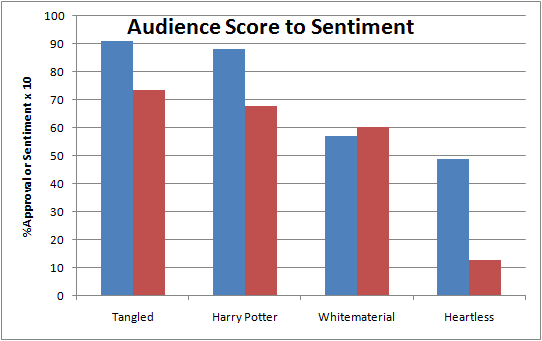
\includegraphics[scale=.55]{img/aatos.png} 
\caption{Audience approval on left, to average excited sentiment score x10 on right}
\label{fig:aapptos}
\end{figure}

When we measure average excited sentiment score against audience approval, another statistic from rotten tomatoes, it removes the issue seen above with the tomato score. This is because the average excited sentiment score does not exhibit the art film effect. It divines the view worthiness of a movie based solely on the approval of the tweeting populace. When matched with audience approval, the coefficient of correlation jumps up to $r=.81$. This indicates that average excited sentiment is an appropriate measure of audience approval.





\subsection{Stocks Analysis}

In order to analyze the data from the tweets we collected on stocks, we compared the tweets per day and the tweet positivity per day with the volume of stocks traded each day, as well as the opening and closing prices of the stocks for each day.  We also charted the daily google trend data for the name of each stock (i.e. the google trends for the word “apple” or the word “microsoft”), but in general this data had little association with both the twitter data and the stock data, probably because Google Trends is limited to one search term.  Overall, these results demonstrated very little correlation, and only the stock volume data appeared to generate any significant correlations with the twitter data.
\begin{figure}[ht!]
\centering
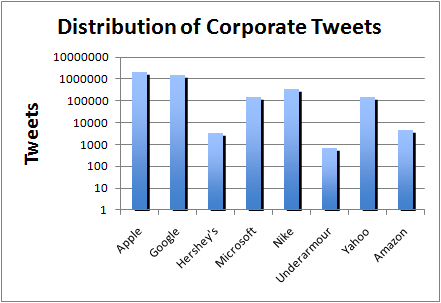
\includegraphics[scale=.65]{img/purestocktweets.png} 
\caption{Distribution of tweets by company}
\end{figure}

Microsoft had entirely negative correlations, the highest of which was the correlation between the number of tweets each day and the volume of stock traded on that day, at $r=-.496$.  While this is still not a very high correlation, the negativity is still interesting. This may be seen in Figure \ref{fig:micvol} This means that the less tweets there are about microsoft, the higher its stock volume is.  This could imply that most tweets about microsoft are complaints, which would mean less people are interested in buying the stock or its products, but since all of microsoft’s daily positivity scores are greater than one, this theory would go against our sentiment analysis of microsoft.  Overall, this is probably just due to the limitations of our data, so it probably means we needed to include more microsoft-related search terms in order to have more effective data.

\begin{figure}[ht!]
\centering
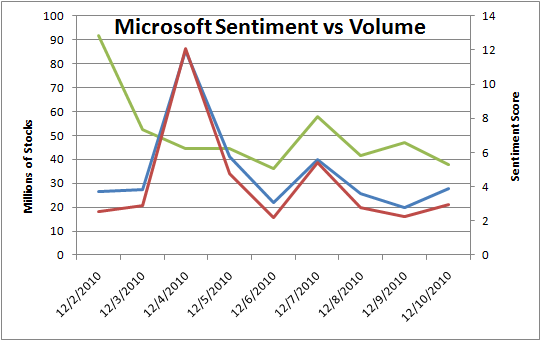
\includegraphics[scale=.55]{img/micvol.png} 
\caption{Microsoft stock volume top, excited sentiment score middle, basic sentiment score bottom }
\label{fig:micvol}
\end{figure}

Overall, the majority of correlations for Google, Yahoo, Microsoft, Hershey’s, Nike, and Under Armour were insignificantly small, so there is no real correlation between the performance of these stocks and their number or positivity of tweets based on the search terms we used.  This could potentially be fixed with better search terms (for example, the Under Armour search term “cold gear” probably generated a lot of noise, considering this study was done in December, and many important words were left off our list, such as macbook for apple), and a more refined method of searching, but overall it seems that twitter is not an effective method of predicting most stocks,(in such a small window) and it is definitely nowhere near as effective in comparison to its ability to predict movie popularity.  Both Yahoo and Hershey’s had a decent negative correlation between positivity from the previous day and stock volume as may be seen in Figure \ref{fig:yahvol} (Excited $r=-.67$, Basic $r=-.588$ for Hershey’s; Excited $r= -.692$, Basic $r=-.610$ for Yahoo), but it is unclear what this means in terms of the relationship between twitter sentiment and stock volume.  It would seem that the more positive sentiment there is for these stocks on twitter, the less likely it is that these stocks are traded, but this result is probably not very reliable because both of these stocks had rather ineffective search terms.  Yahoo had a very small number of search terms overall, while the Hershey’s list included the word “chocolate”, which could be associated with any chocolate company, and so would certainly generate some noise.

\begin{figure}[ht!]
\centering
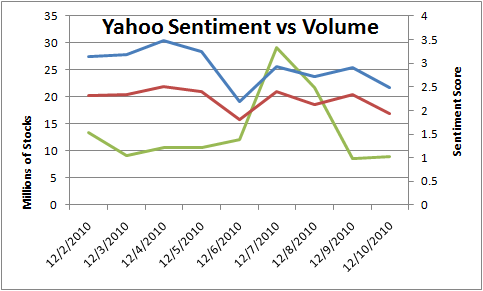
\includegraphics[scale=.55]{img/yahvol.png} 
\caption{Yahoo stock volume top, excited sentiment score middle, basic sentiment score bottom }
\label{fig:yahvol}
\end{figure}

However, both Apple and Amazon generated fairly decent correlation results, although they still did not compare with the correlation between twitter and our movie data.  For Amazon, the excited positivity score correlated well in all time frames (as seen in Figure \ref{fig:amavol}), and the basic positivity had decent correlation as well, indicating that the more positively people feel about Amazon, the more likely they are to trade Amazon stock.  Especially of note is the $r=.644$ correlation between the volume traded and the excited positivity from the day after.  This would indicate that people are more likely to tweet positively about Amazon after they buy its stock, possibly an (probably unconscious) attempt to promote the stock in order to drive the price up.  Apple did not have as many strong correlations as Amazon, but it is interesting that the correlation between the basic positivity score and the volume traded next day is $r=.635$.  While this is not a very strong correlation, it is still strong enough to merit attention.  Based on this correlation, as the amount of positive tweets increases per day, the amount of stocks traded the next day increases.  This is important, because it means that when Apple gets more positive recognition on twitter, it also sells more stock, and so perhaps this value could be used for predicting apple stocks.

\begin{figure}[ht!]
\centering
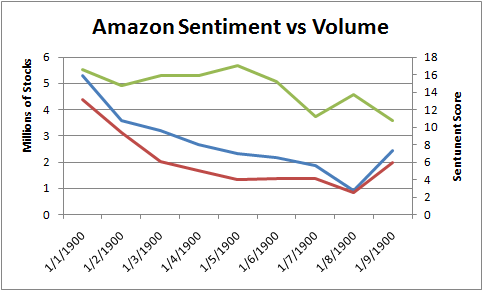
\includegraphics[scale=.55]{img/amavol.png} 
\caption{Amazon stock volume top, excited sentiment score middle, basic sentiment score bottom }
\label{fig:amavol}
\end{figure}


Unfortunately, the overall predictive capabilities of our algorithm are very poor (in other words, I wouldn’t put much stock in it), so it does not seem like there is a very reliable relationship between twitter and stock trading.  Overall, these disappointing results could be due to a number of factors, such as inadequate or unreliable search terms, a less-than-perfect sentiment analysis algorithm, or even the fact that all of our data is slightly skewed by the fact that it was collected in December when many people are still Christmas shopping.  However, the most likely problem is that twitter just is not a good indicator of stock performance, mostly because stocks are affected by so many factors and are so unpredictable that the amount of buzz they get on twitter is not likely to relate to how well they do, especially since our stock terms simply are not as popular on twitter as our movie terms were.  While this data provided interesting insights into how much various companies are talked about on twitter, in terms of predictability, it was ultimately unsuccessful.
\section{Future Work}
In addition to the analyses we have already performed, there are many other methods that could be used in the future to further improve the accuracy and usefulness of this data.  For example, one such improvement that would be useful to implement in the future would be the implementation of a part of speech tagger for the tweet data.  Because the subjective word from "The Subjectivity Lexicon" list also includes a part of speech tag for each word, this method would allow us to categorize only the tweets whose subjective words match the part of speech of "The Subjectivity Lexicon's" word.  For example, while the word \textit{cool} is not in "The Subjectivity Lexicon," but if it were, it would presumably only be included as a positive adjective (as in \textit{that's really cool}).  However, in the methods we used for this analysis, the noun form of cool (as in \textit{it's cool outside}) would also be counted as positive, even though this word is really more likely to be neutral, or possibly even negative.  In "The Subjectivity Lexicon," this is also shown by the word \textit{bullies}, which can be either a noun or verb.  According to the list, both words are negative, so this doesn't affect the sentiment analysis much, but not all cases of homonyms work out so well.

Another improvement we could make in future analysis would be to implement a more effective negation algorithm.  While our negation algorithm is able to handle all cases of the form \textit{not $<$subjective word$>$}, this still leaves out many instances of negation, such as \textit{not $<$non-subjective word$>$ $<$subjective word$>$} or situations in which not is in the form of a conjunction, such as \textit{don't} or \textit{can't}.  However, implementing solutions to these problems without overcorrection (such as making the phrase \textit{not just good, but great} negative when it is clearly positive) is very complicated, and so the best way to implement this would probably be to use a supervised algorithm such as the one proposed by Go et. al.\cite{go-distant}   This supervised algorithm would also be useful for general, non-negated subjectivity as well, as it would allow us to identify other words that influence subjectivity that may not have been included in our initial list, which would result in a more accurate classification of the tweets.

Some of the problems in our data are simply due to difficulties in analyzing twitter data in general.  Because twitter does not allow users to search for any information before the most recent 1500 tweets, analysis can only be done on present tweets, so we were only able to gather data from November 16, 2010 to December 11, 2010.  While this works well for the movies we selected to analyze, as the movies were all released within this time frame, this does not allow us to compare our data to twitter data from past movie releases.  This was especially a problem for our situation, as the release of the highly anticipated seventh instalment of Harry Potter certainly skewed our data, and also decreased the amount of competing movies available to analyze in depth (in fact,daily box-office reports of White Material and Heartless were unavailable because these movies did so poorly).  Because of this, our experiment would be much improved if it could be performed over a longer period of time, so different movies could be analyzed, as well as different weeks, which would allow for much more in-depth analysis of the relation between twitter and movie releases.  This would also be useful for the stock data, as our current analysis might not be the most accurate read of the relationship between twitter and stock performance simply due to the occurrence of Black Friday immediately preceding the period of our data collection, which might have had some effect on sales. Essentially, due to our inability to poll past tweets, our data is constantly subject to the effect of current events, which frequently skews the data and interferes with potential correlation, and the only way to fix this is to gather information over a much longer period of time.

Another problem caused by our use of twitter is the fact that twitter users come from all over the world, while the box office data we used only comes from domestic data.  In fact, only 8\% of Americans use twitter, so our twitter data could be affected by foreign tweets, while our box-office data is purely domestic.  While this could be fixed slightly by only analyzing tweets in English, this solution would still include tweets from England and other English-speaking countries, which would still affect our data.  Overall, it seems the global quality of twitter will act as a limitation in most analyses of American situations, including movie releases, presidential popularity, and other events in which the comparison data is limited to the United States.
	

\section{Conclusion}
Throughout the duration of this project we have explored some of the opportunities offered by simple sentiment analysis on microblogging platforms such as Twitter. We have found that sentiment analysis can be a useful tool in determining how the public has received a movie, and possibly in divining some of their mentality for those movies. We feel that there is still some information that could be had from interpreting tweets about companies and their products; however, due to the tracking terms or possibly the period in which we were searching, we were unable to infer very much. There are many opportunities to improve our sentiment analysis, whether it be by tracking public sentiment over a longer window or refining the means by which we analyzed the tweets.  With these improvements, it would be very interesting to use our algorithm to further examine the relationship  between twitter and various other objects subject to a range of sentiment and opinions.  This could include an analysis of sentiment towards individuals, such as the analysis of Obama and McCain presented in O'Connor et. al., as well as other political analyses, similar to the debate analysis presented by Diakopoulos and Shamma.\cite{oconnor-2010}\cite{diakopoulos-2010}  Twitter analysis might also be used to determine the popularity of specific places, such as amusement parks or museums, as well as the popularity of events.  Event analysis could even be used in comparing two events, such as John Stewart and Stephen Colbert's Rally to Restore Sanity and/or Fear in comparison with Glenn Beck's Restoring Honor Rally.  Furthermore, twitter analysis could be used to analyze to popularity of holidays, particularly less popular holidays such as labor day or veteran's day.  Overall, the possibilities for twitter analysis are almost limitless, and the opportunities grow more and more apparent as twitter grows daily.
\section{Acknowledgements}
We would like to thank Brenden Meeder of Carnegie Mellon University, Richard Wicentowski our professor and advisor, and David Opoku and Sam Clark for engaging in the age old tradition of bouncing ideas.
\section{Appendix}
\subsection{Correlations}
\textbf{Stocks}

\textbf{Movies}
\subsection{Synopses of included Movies}
The following brief synopses are taken from RottenTomatoes.com, a popular aggregator of movie reviews written by a diverse set of critics.

\textbf{Harry Potter and the Deathly Hallows-}In this seventh and final installment of the beloved Harry Potter series, Harry faces new troubles; he must collect all of the Horcruxes that the evil Lord Voldemort has left behind. He has no idea where these are and he has to destroy them all, even without the faintest idea how to do so.
 %rotten tomatoes
 
\textbf{Tangled-} Walt Disney Pictures presents "Tangled," one of the most hilarious, hair-raising tales ever told. When the kingdom's most wanted-and most charming-bandit Flynn Rider (voice of Zachary Levi) hides out in a mysterious tower, he's taken hostage by Rapunzel (voice of Mandy Moore), a beautiful and feisty tower-bound teen with 70 feet of magical, golden hair. Flynn's curious captor, who's looking for her ticket out of the tower where she's been locked away for years, strikes a deal with the handsome thief and the unlikely duo sets off on an action-packed escapade, complete with a super-cop horse, an over-protective chameleon and a gruff gang of pub thugs. In theaters this holiday season in Disney Digital 3D(TM), "Tangled" is a story of adventure, heart, humor and hair-lots of hair. -- (C) Disney

\textbf{Heartless-} Jim Sturgess (21, ACROSS THE UNIVERSE) leads a hugely-talented ensemble cast in this sublime British psychological thriller from cult UK director Philip Ridley (THE REFLECTING SKIN, THE PASSION OF DARKLY NOON), who returns to the screen after a 14-year absence. The film follows Jamie Morgan (Sturgess), born with a disfiguring birthmark across his face, which leaves him an outcast in rough East London. While wandering abandoned yards taking photographs, he comes across a gang of thugs and soon discovers that they are something other than human. He then is led into a Faustian deal that will see him become a party to the terrifying chaos around him. Part DONNIE DARKO, part Guillermo del Toro, this dark urban tale takes its audience to the darkest and most violent corners of the human heart. The film also stars Clémence Poésy, Noel Clarke, Joseph Mawle, Eddie Marsan, Luke Treadaway and Timothy Spall, and was produced by Pippa Cross and Richard Raymond. The film recently won the Best Independent Film Award at the Toronto After Dark Festival. --© IFC

\textbf{White Material-} From Claire Denis, the incomparable director of BEAU TRAVAIL, L'INTRUS and 35 SHOTS OF RHUM, comes WHITE MATERIAL: a rich and thrilling account of a woman driven to the edge. An official selection of the Venice, Toronto and New York Film Festivals, the film is a riveting exploration of the complexities of racial conflict and the limits of human will. The legendary Isabelle Huppert (LA CEREMONIE, THE PIANO TEACHER, 8 WOMEN), is Maria Vial, a fearless French woman attempting to run her family's coffee plantation in an unnamed African country. Torn violently apart by hate-fueled civil conflict, this unforgiving setting soon turns against the foreign family, declaring them outlaws in their new home. In a brash effort to save her family and livelihood, Maria risks everything, fighting with every shred of her will to buck the rebel forces wrestling for control of local power. --© IFC

%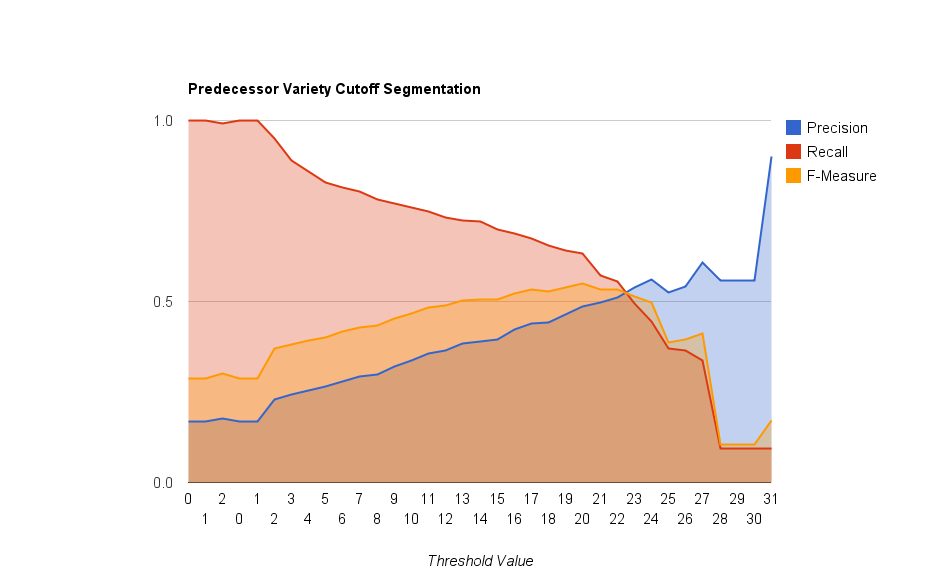
\includegraphics{img/PredVarietyChart.png}
%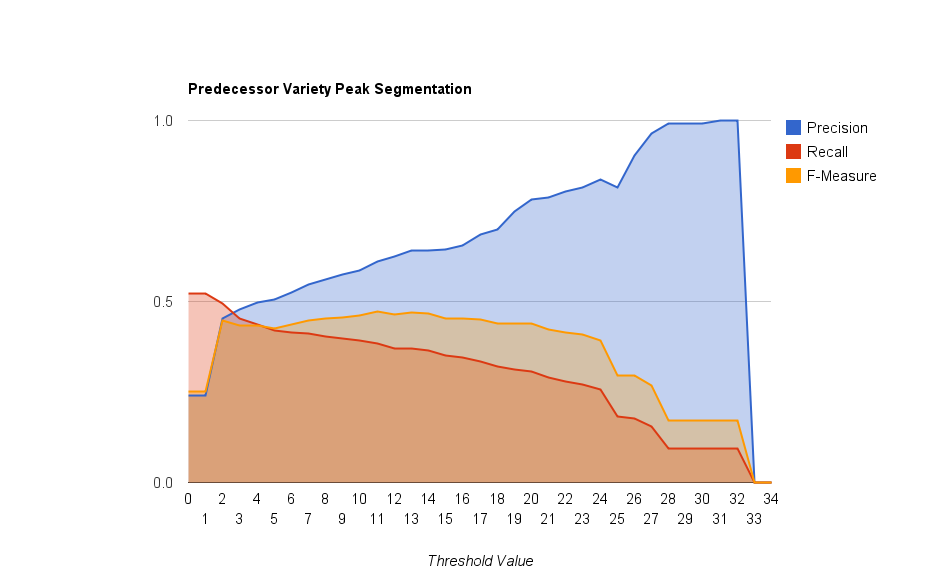
\includegraphics{img/PredVarPeak.png}
%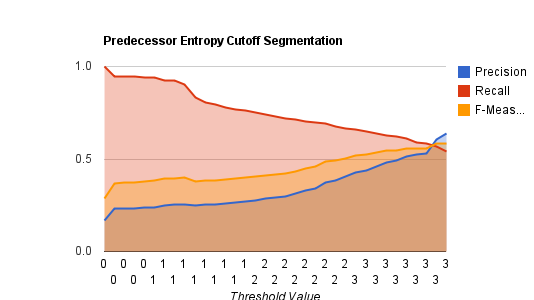
\includegraphics{img/PredEntCutoff.png}
%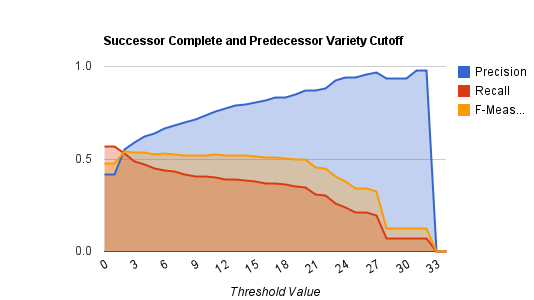
\includegraphics{img/SucCompandPredCut.png}
%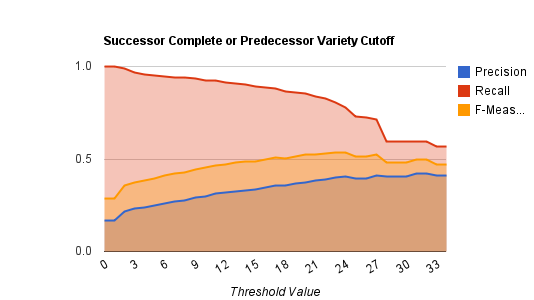
\includegraphics{img/SucComporPredCut.png}
\newpage
\subsection{Graphs and Tables}
\begin{figure}[ht!]
\centering
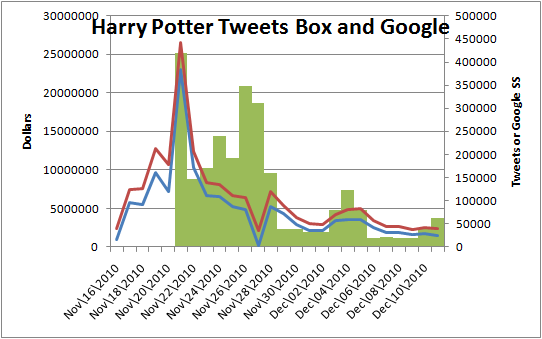
\includegraphics[scale=.55]{img/harrygoog.png} 
\caption{Google Search Score above, Tweet Throughput below, Box as column in background}
\label{fig:harrygoog}
\end{figure}
\begin{figure}[ht!]
\centering
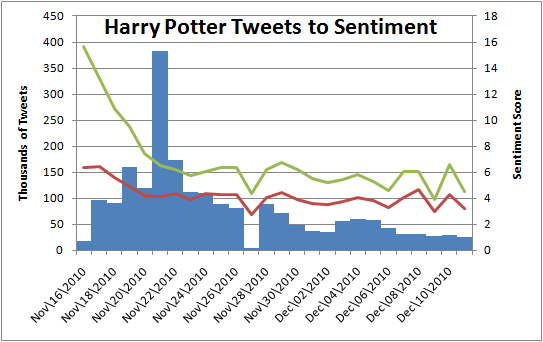
\includegraphics[scale=.55]{img/hptweetsent.png} 
\caption{Tweet Throughput in background, excited score above basic below.}
\label{fig:harrytweetsent}
\end{figure}
\begin{figure}[ht!]
\centering
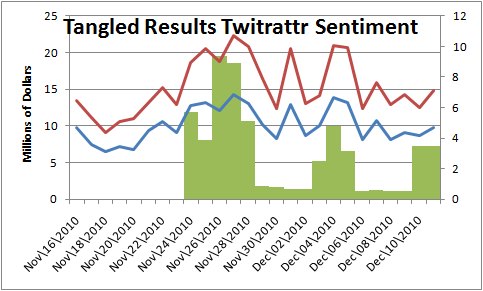
\includegraphics[scale=.55]{img/twitrattr.png} 
\caption{Tweet Throughput in background, excited score above basic below.}
\label{fig:twitrattr}
\end{figure}

\begin{table*}[ht!]
\centering
\caption{Movie Tracking Terms}
\begin{tabular}{|l|c|}
\hline
 Movie & Tracking Terms \\
\hline
Tangled& tangled, pixar \\
\hline
Harry Potter &harry potter, harry potter 7, hp7, deathly hallows\\
\hline
White Material & white material, isabelle huppert\\
\hline
Heartless &heartless, sturgess\\
\hline
\end{tabular}
\label{trackmov}
\end{table*}

\begin{table*}[ht!]
\centering
\caption{Stock Tracking Terms}
\begin{tabular}{|l|c|}
\hline
 Company & Tracking Terms \\
\hline
Apple& AAPL, Apple, ipod, ipad, iphone, imac, mac, steve jobs \\
\hline
Google &GOOG, google, android, droid, chrome, nexus s, gmail, google docs, adwords\\
\hline
Yahoo &YHOO, yahoo, ymail\\
\hline
Microsoft & MSFT, microsoft, steve balmer, windows phone, windows 7, w7, ms\\
\hline
Hershey's&HSY, chocolate, hershey's, hershey park, hersheypark \\
\hline
Amazon &AMZN, amazon.com, amazon\\
\hline
Nike & NKE, nike, shoes, nikes, swoosh, just do it\\
\hline
Under Armour &UA, underarmour, under armour, protect this house, heat gear, cold gear\\
\hline
\end{tabular}
\label{trackst}
\end{table*}

\newpage
\pagebreak[4]
\bibliographystyle{cs65f10}
\bibliography{cs65f10}

\end{document}
